\documentclass[10pt]{beamer}

\usetheme{metropolis}
\usepackage{appendixnumberbeamer}

\usepackage{tikz}
\usetikzlibrary{shapes.geometric, arrows} 
\usetikzlibrary{positioning} % <-- ESSA LINHA É A QUE CORRIGE O ERRO

\usepackage{booktabs}
\usepackage[scale=2]{ccicons}

\usepackage{pgfplots}
\usepgfplotslibrary{dateplot}

\usepackage{xspace}
\newcommand{\themename}{\textbf{\textsc{metropolis}}\xspace}

% CONFIGURAÇÃO DO TEMA METROPOLIS
 
\usepackage[utf8]{inputenc}
\usepackage[T1]{fontenc}
\usepackage[portuguese]{babel}
\usepackage{fontspec}

% Pacotes Adicionais (Recomendados para visualizações)
\usepackage{amsmath}
\usepackage{amsfonts}
\usepackage{amssymb}
\usepackage{booktabs}
\usepackage{caption}
\usepackage{ragged2e} % Para justificar texto (se necessário)

% FONTES (These commands require XeLaTeX/LuaLaTeX and the fontspec package)
 \setsansfont{Fira Sans Light}[Scale=MatchLowercase]
 \setmainfont{Fira Sans}[Scale=MatchLowercase]
 \setmonofont{Noto Sans Mono}[Scale=MatchLowercase]

% --- INFORMAÇÕES DO APRESENTADOR ---
\title{NECTA: Neural Electrophysiological Connectivity Time-resolved Analysis} 

% Subtítulo (opcional, foco do doutorado)
\subtitle{Uma Plataforma para Análise do Dinoma e Conectividade Efetiva}

\author{Jaime B. Cirne de Oliveira, }

\institute{
    Laboratório de Neurobiologia da Visão, Instituto do Cérebro, UFRN, Brasil
     
}
\date{\today}

% --- INÍCIO DO DOCUMENTO ---
\begin{document}

% SLIDE 1: TÍTULO
\maketitle



% ==================================================================================================================
\section{I. O Desafio de Compreender a Dinâmica Cerebral}
% ==================================================================================================================

\begin{frame}{O Paradoxo Analítico}
    \centering
    \vspace{1.5cm}
    
    \Large \textbf{Resolução vs. Representação}
    
    \vspace{1cm}
    \normalsize
    Registramos a atividade cerebral com precisão de milissegundos, mas ainda a analisamos predominantemente através de \textbf{representações estáticas}.
\end{frame}

\begin{frame}{A Limitação do Paradigma Estático}
    \begin{columns}[c]
        \begin{column}{0.4\textwidth}
            \textbf{A Falsa Premissa Estática}
            \vspace{0.3cm}
            \begin{itemize}
                \item Foco em redes com conexões fixas.
                \item O mapeamento estrutural não descreve o \textbf{fluxo direcional e dinâmico} de informação.
            \end{itemize}
        \end{column}
        \begin{column}{0.55\textwidth}
            \centering
            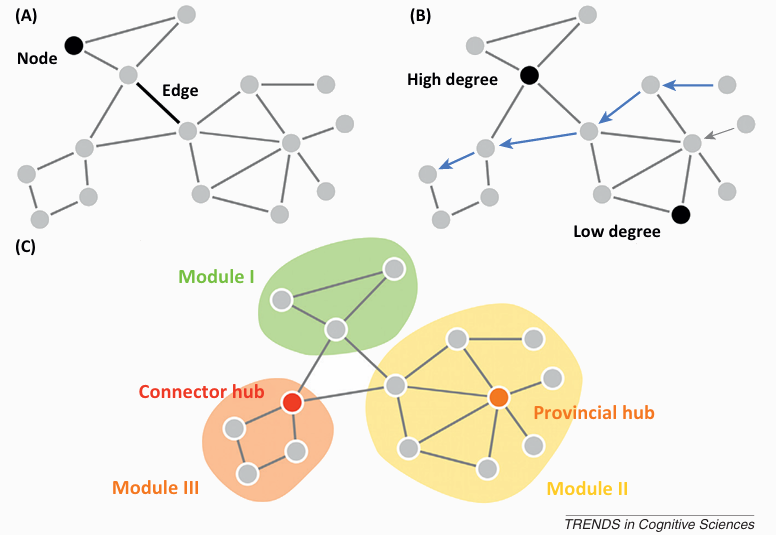
\includegraphics[width=0.9\textwidth]{./imgs/Figura1_Sporns.png}
            \captionof{figure}{\tiny Representação Estática. \textit{Fonte: Van den Heuvel \& Sporns (2013).}}
        \end{column}
    \end{columns}
\end{frame}

\begin{frame}{A Necessidade do Dinoma}
    \begin{columns}[c]
        \begin{column}{0.48\textwidth}
            \centering
            \Large \textbf{Conectoma} \\
            \normalsize (Estático)
            
            \vspace{0.6cm}
            O mapa estrutural subjacente.
        \end{column}
        \begin{column}{0.48\textwidth}
            \centering
            \Large \textbf{Dinoma} \\
            \normalsize (Dinâmico)
            
            \vspace{0.6cm}
            A rápida reconfiguração direcional no tempo.
        \end{column}
    \end{columns}
\end{frame}

\begin{frame}{O Gargalo Analítico}
    \centering
    \vspace{1cm}
    
    \Large \textbf{A Explosão Computacional}
    
    \vspace{1cm}
    \normalsize
    Mapear o fluxo de informação causal ao longo de milhares de janelas temporais gera um \textbf{volume massivo e intratável} de dados por métodos convencionais.
    
    \vspace{1.5cm}
    \textit{Como podemos superar esse gargalo para formular e testar hipóteses sobre a dinâmica cerebral?}
\end{frame}

% ==================================================================================================================
\section{II. A Hipótese do Dinoma e Objetivos}
% ==================================================================================================================

\begin{frame}{A Pergunta de Pesquisa}
    \centering
    \vspace{2cm}
    
    \Large
    \textit{"Como o fluxo de informação se reconfigura nas redes corticais durante o processamento visual, e qual o papel da Zona de Transição?"}
\end{frame}

\begin{frame}{A Hipótese Científica}
    \centering
    \vspace{1.5cm}
    
    \Large \textbf{\textit{Hub} Dinâmico Inter-Hemisférico}
    
    \vspace{1cm}
    \normalsize
    A \textbf{Zona de Transição (TZ)} não é apenas uma fronteira anatômica, mas atua como o principal roteador direcional de informações durante o processamento do estímulo.
\end{frame}

\begin{frame}{Objetivos da Tese}
    \vspace{0.5cm}
    \begin{itemize}
        \item \textbf{Geral:} Investigar a dinâmica direcional (Dinoma) das redes corticais no tempo.
        \vspace{0.8cm}
        \item \textbf{Específico 1:} Mapear a evolução temporal da integração e segregação da rede.
        \vspace{0.8cm}
        \item \textbf{Específico 2:} Determinar os principais emissores (\textit{drivers}) e receptores (\textit{sinks}) de fluxo causal, identificando \textit{hubs} dinâmicos.
    \end{itemize}
\end{frame}

\begin{frame}{Contribuições Esperadas}
    \begin{alertblock}{Compreensão do Dinoma}
        Evidenciar empiricamente que as redes cerebrais alternam rapidamente entre estados estruturados de alta e baixa integração funcional.
    \end{alertblock}
    
    \vspace{0.5cm}
    \begin{alertblock}{O Papel da Zona de Transição}
        Caracterizar a função direcional da TZ, preenchendo uma lacuna na compreensão da comunicação cortical inter-hemisférica.
    \end{alertblock}
\end{frame}

\begin{frame}{A Barreira Tecnológica}
    \centering
    \vspace{1.5cm}
    
    \Large \textbf{O Problema da Escalabilidade}
    
    \vspace{1cm}
    \normalsize
    Testar essas hipóteses biológicas exige o cálculo direcional rigoroso em milhares de janelas temporais, gerando um \textbf{volume intratável de dados}.
    
    \vspace{1.5cm}
    \textit{Como podemos viabilizar computacionalmente essa investigação em larga escala?}
\end{frame}


% ==================================================================================================================
\section{III. NECTA: O Instrumento de Descoberta}
% ==================================================================================================================

\begin{frame}{NECTA: O Instrumento de Descoberta}
    \centering
    
    % Figura Principal
    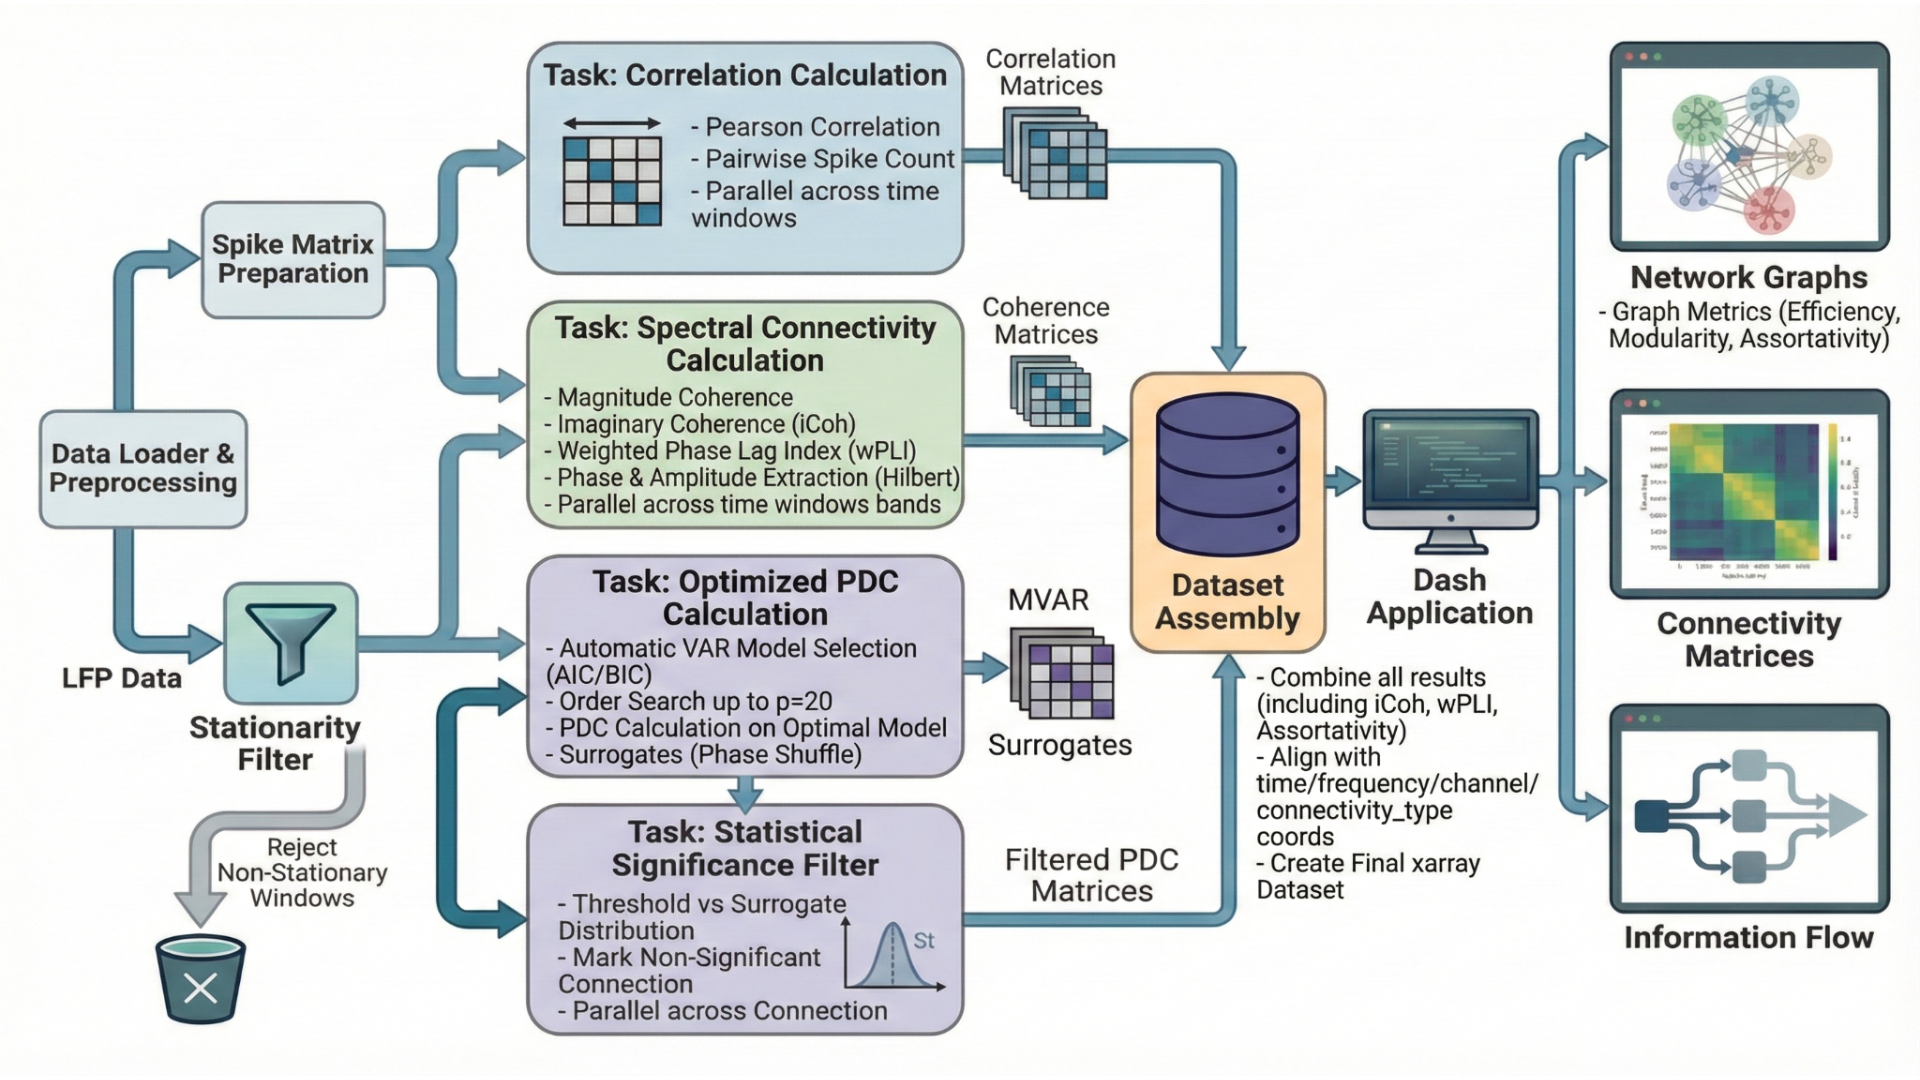
\includegraphics[width=1\textwidth, keepaspectratio]{./imgs/pipeline.png}
    
    \vspace{0.4cm}
    \begin{columns}[T]
        \begin{column}{0.32\textwidth}
            \centering
            \textbf{1. Entrada} \\
            \vspace{0.1cm}
            \small Matrizes densas de sinais eletrofisiológicos.
        \end{column}
        \begin{column}{0.35\textwidth}
            \centering
            \textbf{2. Motor Computacional} \\
            \vspace{0.1cm}
            \small Cálculo direcional distribuído em janelas deslizantes.
        \end{column}
        \begin{column}{0.32\textwidth}
            \centering
            \textbf{3. Saída} \\
            \vspace{0.1cm}
            \small Evolução temporal das redes e \textit{hubs} causais.
        \end{column}
    \end{columns}
    
    \vspace{0.8cm}
    \textit{Mas como garantimos que o mapeamento dinâmico gerado não é mero ruído estatístico?}
\end{frame}% ==================================================================================================================
\section{IV. Validação Computacional: Viabilidade e Rigor}
% ==================================================================================================================

\begin{frame}{Rigor Estatístico}
    \centering
    \vspace{1cm}
    
    \Large \textbf{Separando Sinal de Ruído}
    
    \vspace{0.8cm}
    \normalsize
    O cálculo direcional em milhares de janelas temporais eleva exponencialmente o risco de correlações espúrias. Para garantir a validade biológica, empregamos \textbf{\textit{Surrogate Data} (AAFT)}.
    
    \vspace{0.8cm}
    \begin{alertblock}{Causalidade Fisiológica}
        A geração iterativa de distribuições nulas garante que apenas conexões direcionalmente significativas componham o grafo dinâmico.
    \end{alertblock}
\end{frame}

\begin{frame}{Escalabilidade e Desempenho}
    \centering
    \vspace{1cm}
    
    \Large \textbf{Processamento Paralelo Massivo}
    
    \vspace{1cm}
    \normalsize
    A arquitetura particiona tensores multidimensionais, distribuindo o cálculo de conectividade por múltiplos núcleos de processamento.
    
    \vspace{0.8cm}
    \begin{itemize}
        \item \textbf{Desempenho:} Redução dramática do tempo de execução.
        \item \textbf{Viabilidade:} Permite analisar uma densidade temporal que seria intratável por métodos seriais tradicionais.
    \end{itemize}
\end{frame}

\begin{frame}{Reprodutibilidade Científica}
    \centering
    \vspace{1.5cm}
    
    \Large \textbf{Padronização do Fluxo de Trabalho}
    
    \vspace{1cm}
    \normalsize
    Toda a metodologia opera sob um \textit{framework} modular e reprodutível. Isso assegura que os resultados sejam auditáveis e a abordagem aplicável a novos conjuntos de dados eletrofisiológicos.
\end{frame}

\begin{frame}{A Base para a Descoberta}
    \centering
    \vspace{1cm}
    
    \Large \textbf{Uma Metodologia Confiável}
    
    \vspace{1cm}
    \normalsize
    Ao unir \textbf{rigor estatístico}, \textbf{escalabilidade} e \textbf{reprodutibilidade}, superamos o gargalo analítico e estabelecemos uma base sólida para a inferência neurobiológica.
    
    \vspace{1.5cm}
    \textit{Com essa ferramenta validada, o que o mapeamento dinâmico nos revela sobre o cérebro vivo?}
\end{frame}

% ==================================================================================================================
% ==================================================================================================================
\section{V. Descobertas Biológicas: Mapeando o Dinoma}
% ==================================================================================================================

\begin{frame}{Organização Anatômica da Rede Cortical}
    \centering
    \vspace{0.2cm}
    
    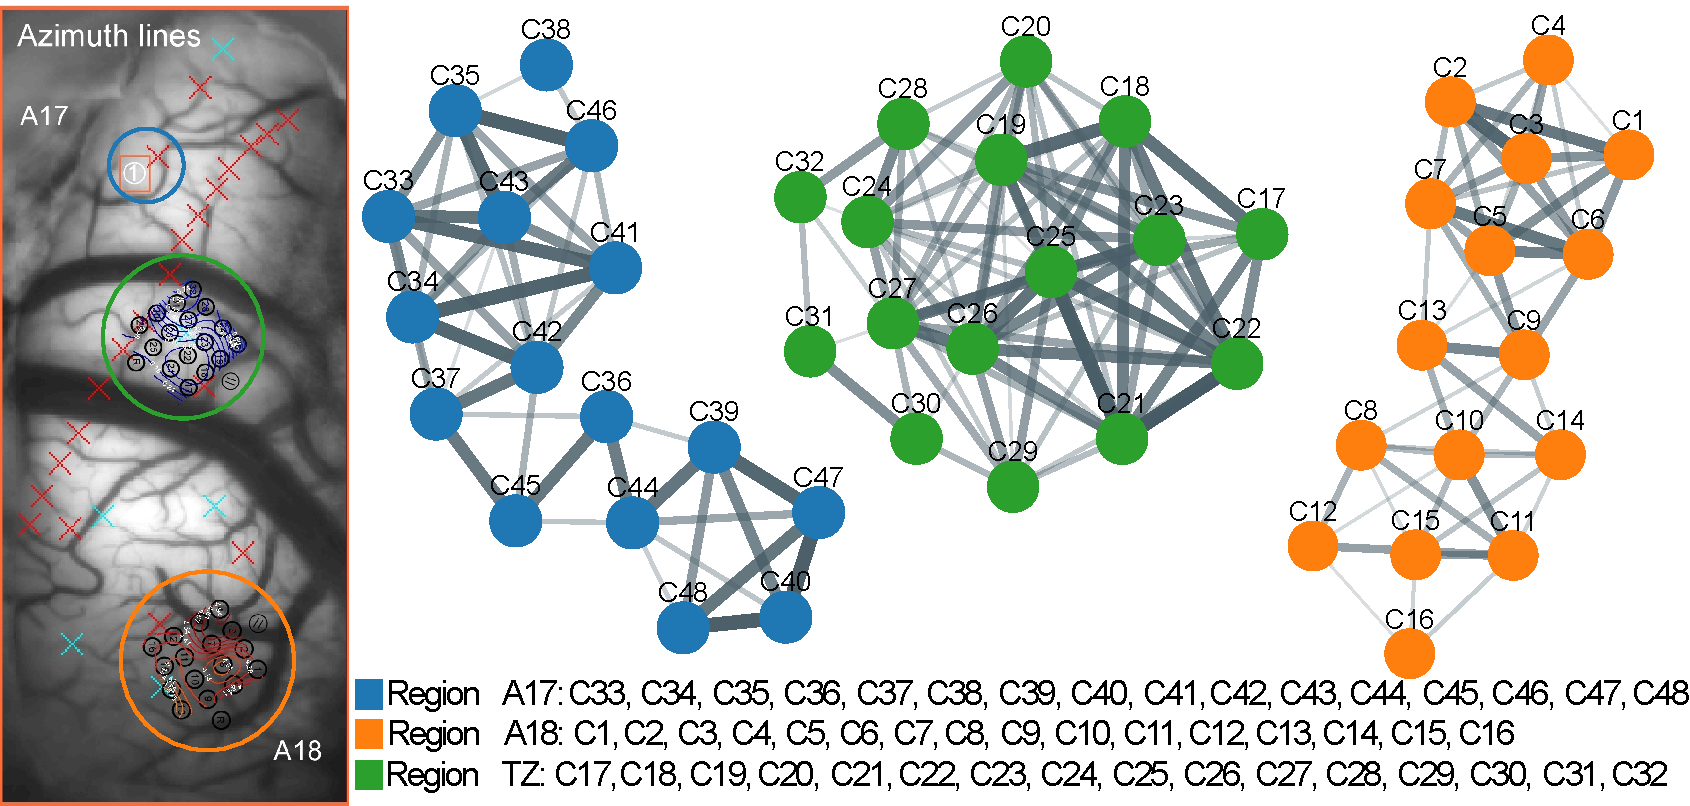
\includegraphics[width=0.95\textwidth, height=0.65\textheight, keepaspectratio]{./imgs/Figura01.pdf}
    
    \vspace{0.4cm}
    \begin{itemize}
        \item Os eletrodos corticais foram organizados em três regiões funcionais principais: \textbf{Área 17}, \textbf{Zona de Transição (TZ)} e \textbf{Área 18}.
        \item Este modelo anatômico estabelece a referência espacial estrita para todas as análises subsequentes de conectividade dinâmica.
    \end{itemize}
\end{frame}

% --- INÍCIO DA HISTÓRIA 1: CONECTIVIDADE NÃO-DIRECIONADA (CORRELAÇÃO / COERÊNCIA) ---

% SLIDE 7 (Antigo 9): Para ilustrar visualmente o Dinoma (Diferença Estático vs. Dinâmico)
\begin{frame}{A Topologia Cortical é Altamente Dinâmica}
    \centering
    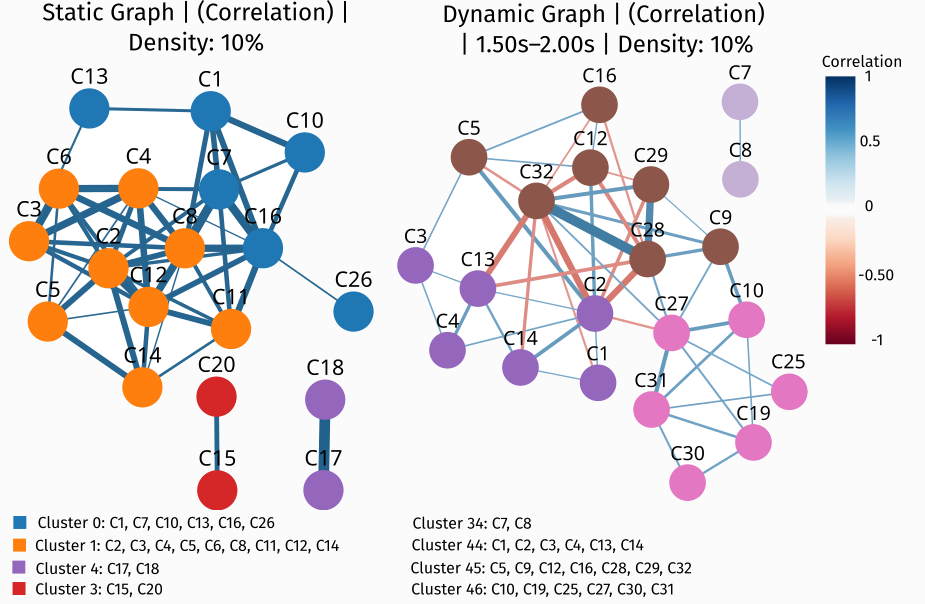
\includegraphics[width=0.9\textwidth]{./imgs/imagem_comparativa.png}
    
    \vspace{0.4cm}
    \begin{alertblock}{Ocultamento Temporal}
        A média temporal estática esconde a profunda reconfiguração da rede causal. O conectoma funcional opera essencialmente em estados transitórios e direcionais.
    \end{alertblock}
\end{frame}

\begin{frame}{Microestados e Organização Temporal}
    \centering
    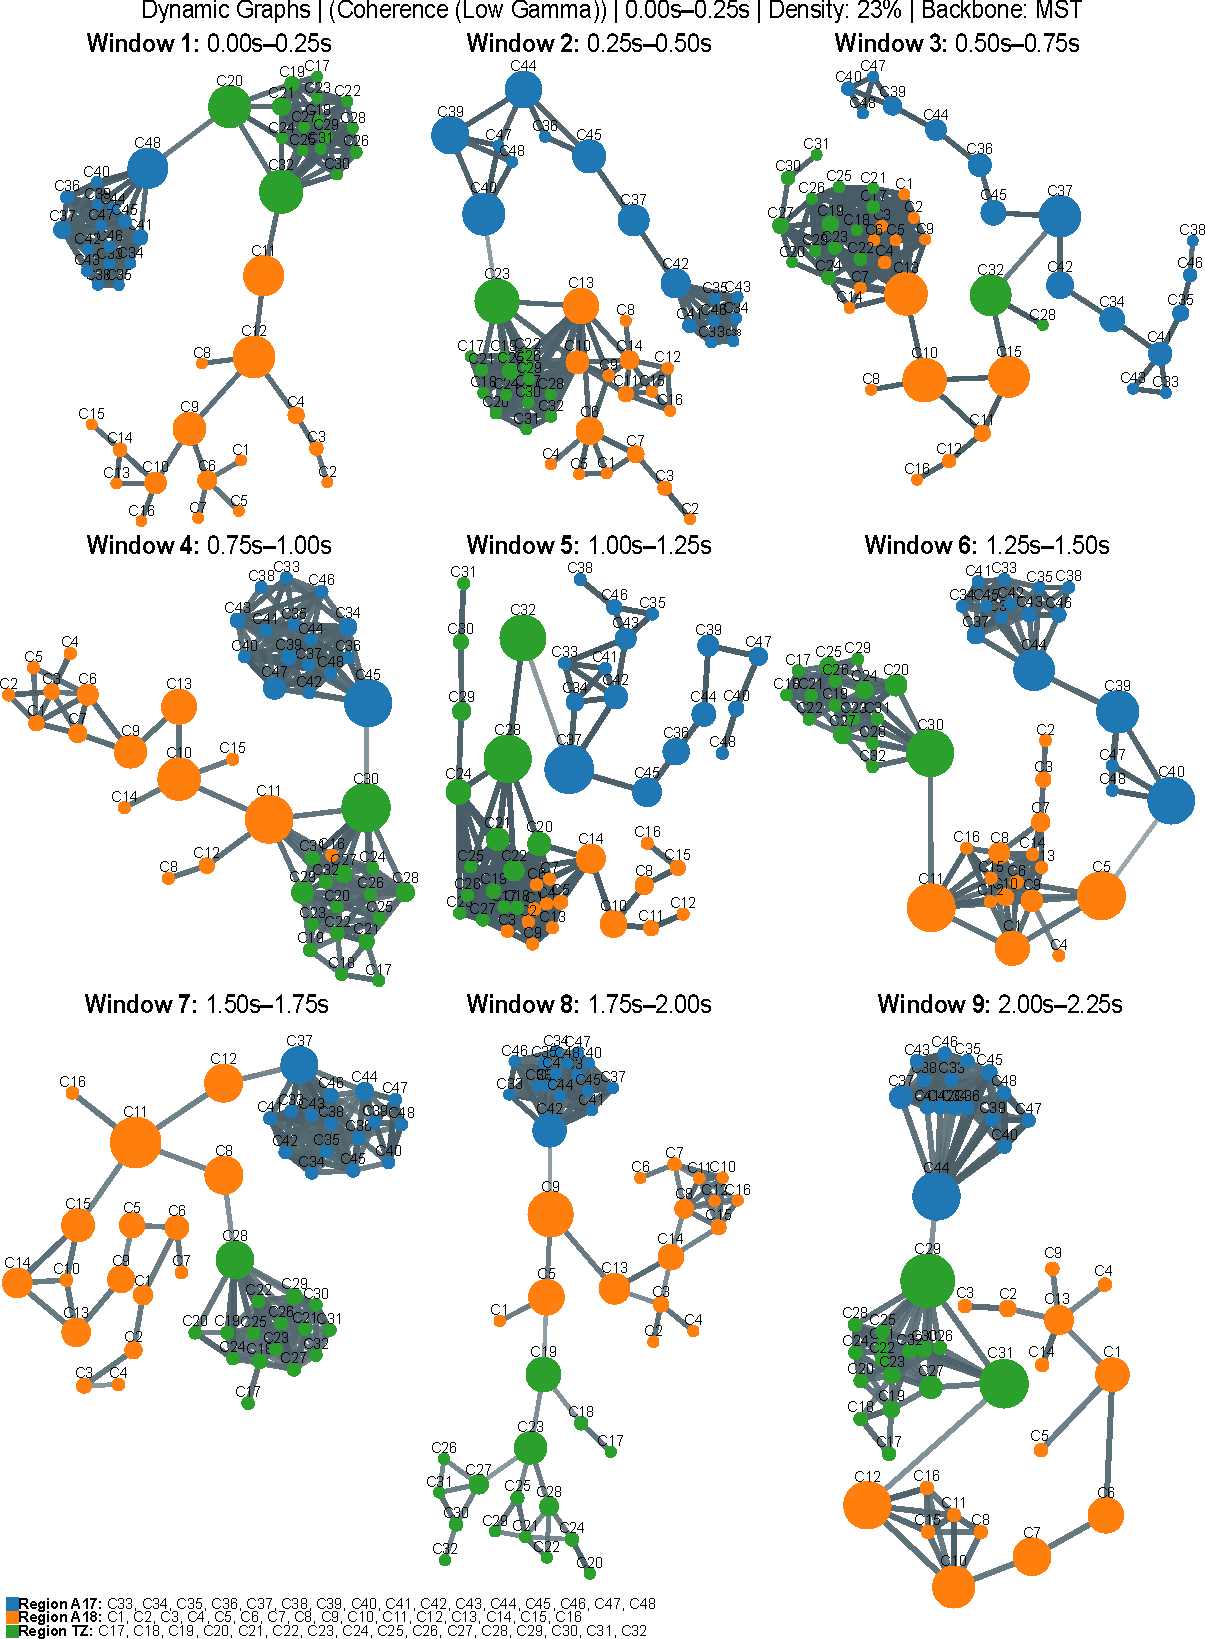
\includegraphics[width=0.95\textwidth]{./imgs/Dynamic Graphs.pdf}
    
    \vspace{0.4cm}
    \begin{alertblock}{Ancoragem Visual}
        A evolução direcional revela transições físicas entre microestados de segregação e integração funcional, fortemente ritmados pelo processamento do estímulo.
    \end{alertblock}
\end{frame}

\begin{frame}{A Reconfiguração da Rede Cortical Pode Ser Quantificada}
    \centering
    \vspace{0.2cm}
    
    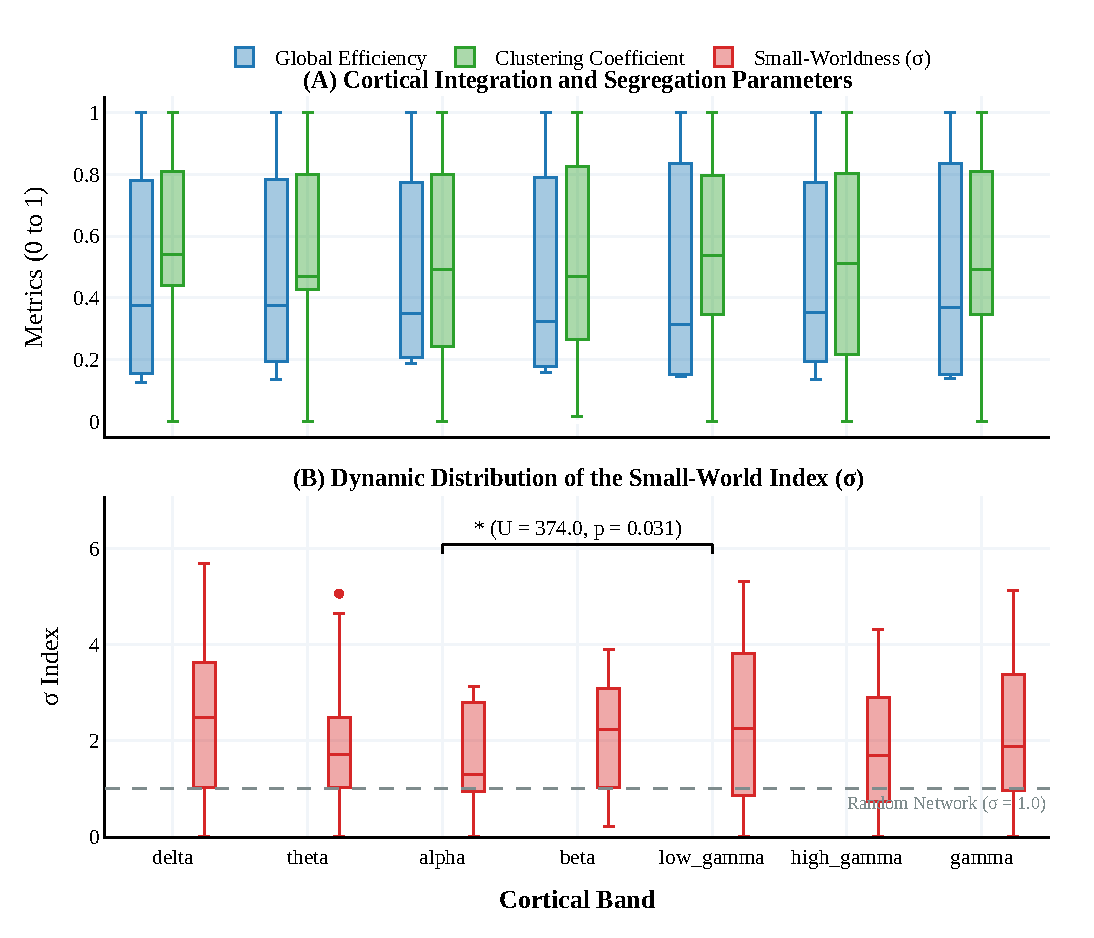
\includegraphics[width=0.95\textwidth, height=0.60\textheight, keepaspectratio]{./imgs/Metricas_NECTA.pdf}
    
    \vspace{0.4cm}
    \begin{itemize}
        \item A Eficiência Global e a Segregação (\textit{Clustering}) revelam quantitativamente as mudanças dinâmicas na organização cortical.
        \item A banda \textit{Low Gamma} exibe a organização \textit{Small-World} mais robusta da rede.
    \end{itemize}
\end{frame}

\begin{frame}{O Estímulo Conduz o Córtex a um Regime \textit{Small-World}}
    \centering
    
    % Figura Principal (~70% da área, com overlay do TikZ)
    \begin{tikzpicture}
        \node[anchor=south west, inner sep=0] (image) at (0,0) {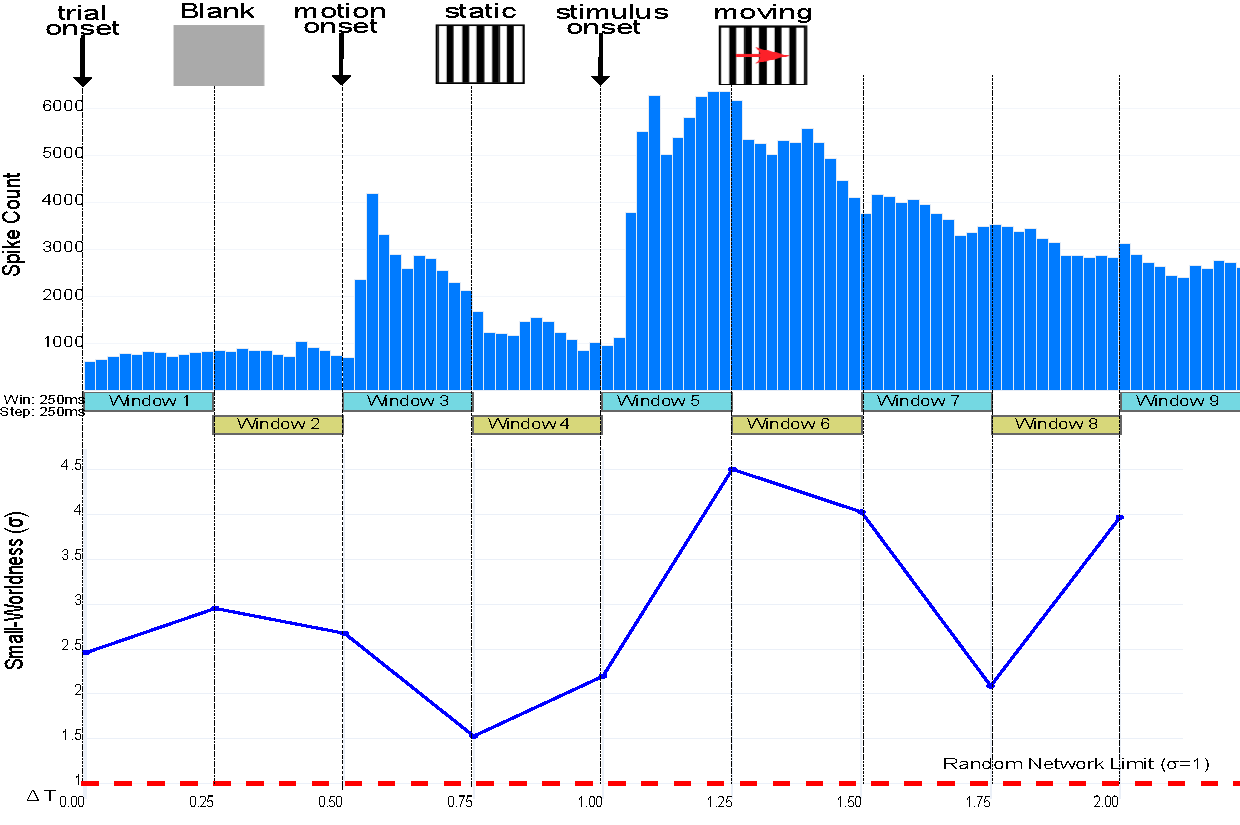
\includegraphics[width=0.95\textwidth, height=0.55\textheight, keepaspectratio]{./imgs/SpikeVsSW.pdf}};
        
        \begin{scope}[x={(image.south east)},y={(image.north west)}]
            % 1. Ocultar labels de implementação ("Window 1...9", "Win/Step") 
            % Localizados na faixa central entre os dois gráficos
            \fill[white] (0.0, 0.46) rectangle (1.0, 0.53);
            
            % 2. Destacar o intervalo de maximização da métrica Small-World (pico do gráfico inferior)
            \fill[yellow, opacity=0.3, rounded corners=2pt] (0.45, 0.05) rectangle (0.65, 0.44);
            \draw[red!80!black, thick, dashed, rounded corners=2pt] (0.45, 0.05) rectangle (0.65, 0.44);
            \node[anchor=south, font=\scriptsize\bfseries, text=red!80!black] at (0.55, 0.44) {Maximização \textit{Small-World}};
        \end{scope}
    \end{tikzpicture}
    
    \vspace{0.2cm}
    \begin{itemize}
        \item A reconfiguração fisiológica atinge um balanço ótimo entre integração global e especialização.
        \item A maximização da topologia \textit{small-world} coincide com a altíssima demanda computacional pós-estímulo.
    \end{itemize}
    
    \vspace{0.1cm}
    \begin{alertblock}{Take-home Message}
        A eficiência neurocomputacional é garantida por rápidas transições dinâmicas e diretas, não por conexões estáticas.
    \end{alertblock}
\end{frame}

\begin{frame}{O Fluxo Direcional Revela os Centros de Controle da Rede}
    \centering
    \textbf{\small A Conectividade Efetiva (PDC) identifica as principais fontes e alvos do fluxo de informação cortical.}
    
    \vspace{0.1cm}
    
\includegraphics[width=0.95\textwidth, height=0.45\textheight, keepaspectratio]{./imgs/PDC_graph.pdf}
    
    \vspace{0.1cm}
    \begin{itemize}
        \item A conectividade efetiva revela a direção da transferência de informação entre regiões corticais.
        \item O balanço do fluxo (\textit{Net Flow}) identifica os emissores (\textit{drivers}) e receptores (\textit{sinks}) dominantes.
    \end{itemize}
    
    \vspace{0.2cm}
    \textit{\small Se o fluxo direcional revela os centros de controle da rede, qual região emerge sistematicamente como o hub dominante?}
\end{frame}

\begin{frame}{O Papel Ativo da Zona de Transição}
    \justifying
    \vspace{1cm}
    
    O mapeamento direcional de alta densidade revelou o verdadeiro papel da \textbf{Zona de Transição (TZ)}, antes tratada como uma mera fronteira anatômica.
    
    \vspace{0.6cm}
    \begin{alertblock}{\textit{Hub} de Roteamento Inter-Hemisférico}
        \begin{itemize}
            \item A TZ sustenta um trânsito causal (\textit{Net Flow}) altíssimo e volátil no decorrer do estímulo.
            \item Em janelas temporais de pico integrativo, a capacidade de roteamento da TZ supera a das próprias áreas sensoriais primárias (e.g., Área 18).
            \item \textbf{Descoberta:} A TZ funciona ativamente como um \textit{hub} integrador fundamental para a coordenação cortical bilateral rápida.
        \end{itemize}
    \end{alertblock}
\end{frame}

% ==================================================================================================================
\section{VI. Contribuições da Tese}
% ==================================================================================================================

% SLIDE 1: Contribuições Alcançadas
\begin{frame}{O Impacto Científico da Tese}
    \justifying
    O presente trabalho entregou contribuições originais e concretas em três pilares fundamentais da pesquisa neurocientífica:
    
    \vspace{0.3cm}
    \begin{alertblock}{1. Contribuição Computacional}
        Resolução do gargalo analítico por meio de uma arquitetura escalável, viabilizando o cálculo massivo e em tempo hábil da conectividade direcional em alta densidade temporal.
    \end{alertblock}

    \vspace{0.1cm}
    \begin{alertblock}{2. Contribuição Metodológica}
        Estabelecimento e validação estatística rigorosa de um fluxo analítico (janelas deslizantes + AAFT) para o mapeamento dinâmico causal de sinais eletrofisiológicos brutos.
    \end{alertblock}

    \vspace{0.1cm}
    \begin{alertblock}{3. Contribuição Biológica}
        Demonstração empírica da rápida reconfiguração topológica do fluxo de informação (\textit{O Dinoma}) e a redefinição funcional das fronteiras corticais (Zona de Transição).
    \end{alertblock}
\end{frame}


% ==================================================================================================================
\section{VII. Conclusões e Próximos Passos}
% ==================================================================================================================

\begin{frame}{Síntese da Tese}
    \centering
    \vspace{0.5cm}
    
    \begin{columns}[T]
        \begin{column}{0.45\textwidth}
            \textbf{O Problema} \\
            \small A ausência de metodologias para mapear o fluxo causal de informações em larga escala e alta resolução temporal.
            
            \vspace{0.5cm}
            \textbf{A Solução} \\
            \small Um \textit{framework} computacional robusto, determinístico e validado estatisticamente para inferência dinâmica.
        \end{column}
        
        \begin{column}{0.45\textwidth}
            \textbf{As Descobertas} \\
            \small A comprovação empírica do \textit{Dinoma} e a redefinição das fronteiras corticais como \textit{hubs} integrativos.
            
            \vspace{0.5cm}
            \textbf{O Impacto} \\
            \small Uma nova lente biológica e computacional capaz de redefinir nossa compreensão sobre as redes funcionais do cérebro.
        \end{column}
    \end{columns}
\end{frame}

\begin{frame}{Perspectivas e Trabalhos Futuros}
    \justifying
    \vspace{0.3cm}
    Para a conclusão do doutorado, as seguintes frentes de pesquisa serão priorizadas:
    
    \vspace{0.6cm}
    \begin{itemize}
        \setlength\itemsep{0.5cm}
        \item \textbf{1. Acurácia Anatômica:}\\
        Registro espacial preciso dos canais para enriquecer a interpretação biológica das vias mapeadas.
        \item \textbf{2. Modulação Sensorial:}\\
        Investigação da resiliência e flexibilidade da rede dinâmica sob estímulos com diferentes frequências espaciais.
        \item \textbf{3. Impacto Translacional:}\\
        Avaliação do \textit{Dinoma} causal como um possível neuromarcador de alta precisão para patologias neurodegenerativas.
    \end{itemize}
\end{frame}

\begin{frame}[standout]
    A transição da conectividade estática para a rede causal dinâmica representa uma quebra de paradigma na compreensão da fisiologia do cérebro vivo.\\
    \vspace{1.2cm}
    \textbf{Muito Obrigado.}\\
    \vspace{0.8cm}
    \normalsize Dúvidas e Discussões?
\end{frame}

\end{document}
